% !TeX spellcheck = en_US

\chapter{Practical Results}\label{chp:practical_results}

\section{QGIS Plugin}
A QGIS plugin was created in this research. It allows the processing of currently displayed imagery in a corresponding backend server. \autoref{fig:plugin:changes} shows an image of the imagery layer overlaid with the changes generated by the backend. The red dots on the upper left indicate deleted objects – that is, buildings which were not predicted in the image but existed at the same location in the cadastral survey data. However, in this case the neural network was incorrect because the actual buildings can be seen clearly. Additionally, in the lower middle area, a blue region can be seen which indicates a change in the survey data. A prediction is classified as a change as soon as it fully covers at least one existing object in the survey data. \autoref{fig:plugin:changes_cadastral_layer} shows the same changes on the cadastral data layer, and \autoref{fig:plugin:predictions} shows the predictions returned by the neural network.

\begin{figure}[H]
    \centering
	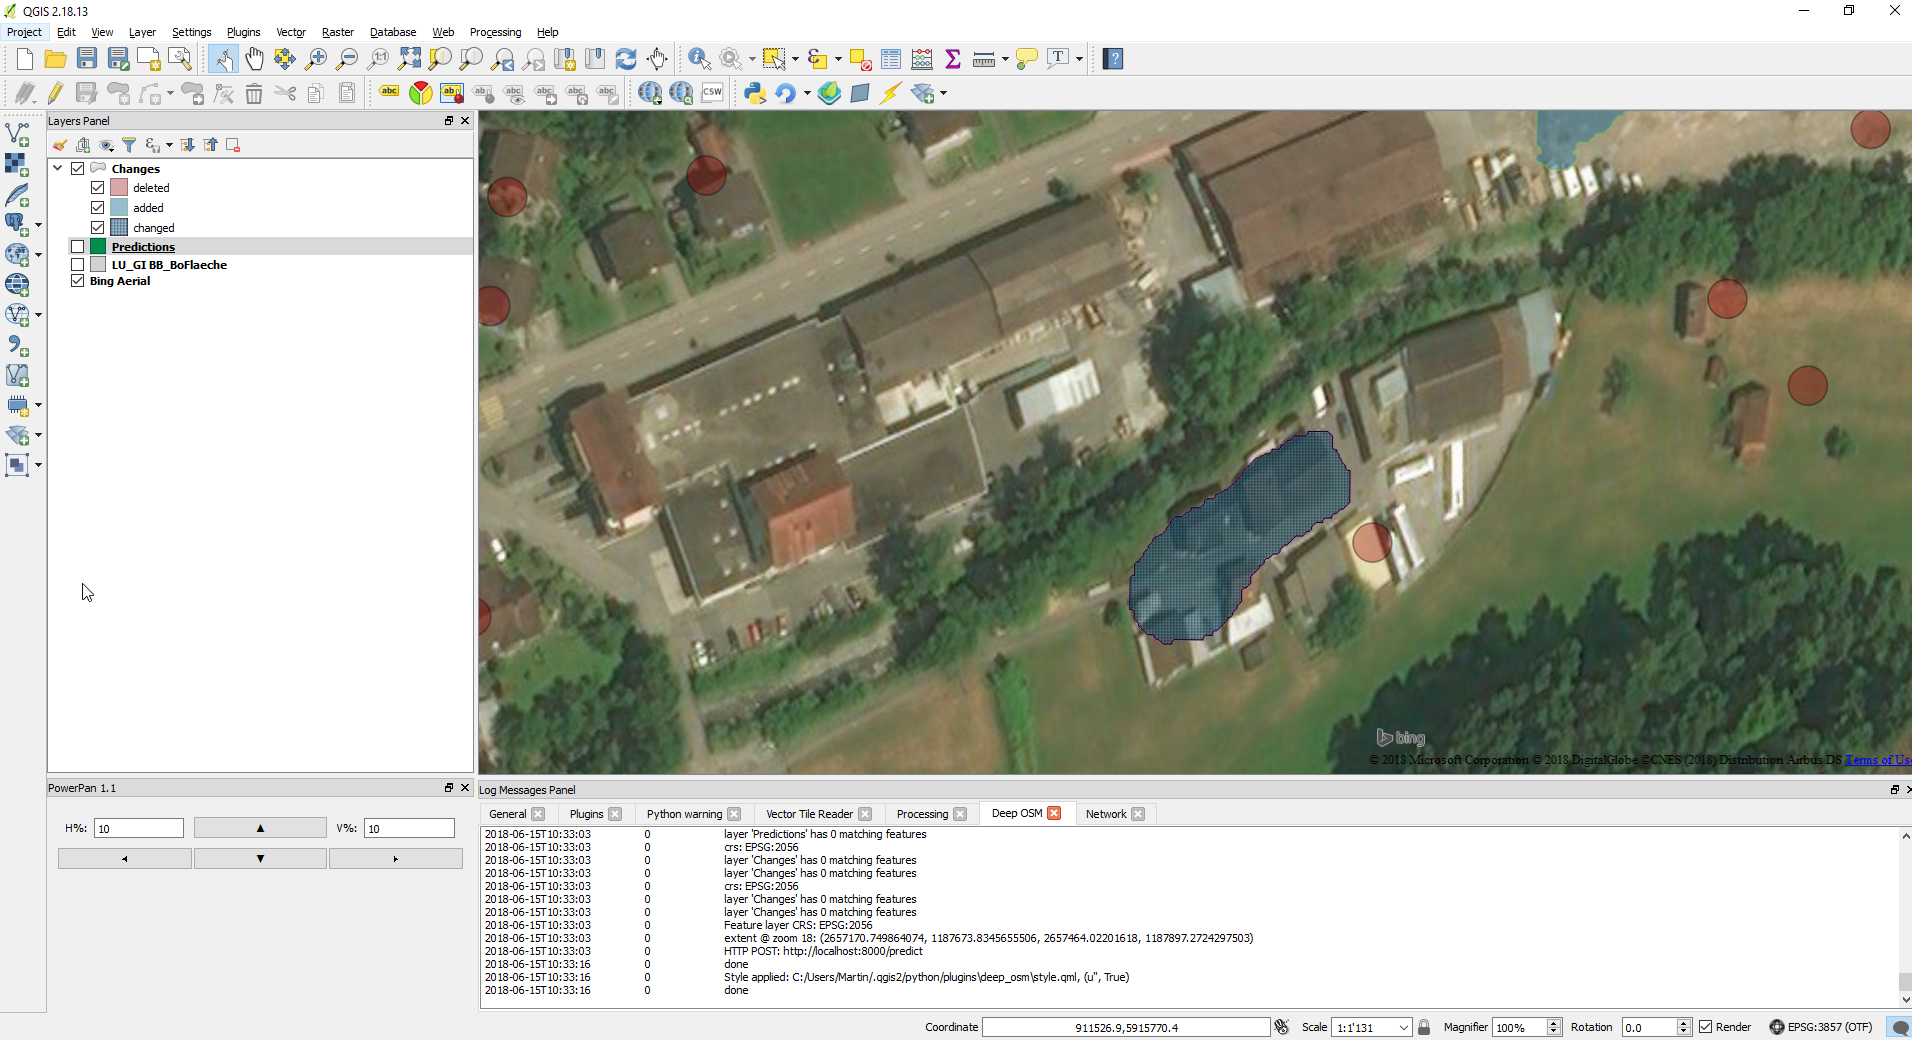
\includegraphics[width=1\linewidth]{chapters/practical_results/images/qgis_changes_aerial.png}
	\caption{Changes in QGIS}
	\label{fig:plugin:changes}
\end{figure}

\begin{figure}[H]
    \centering
	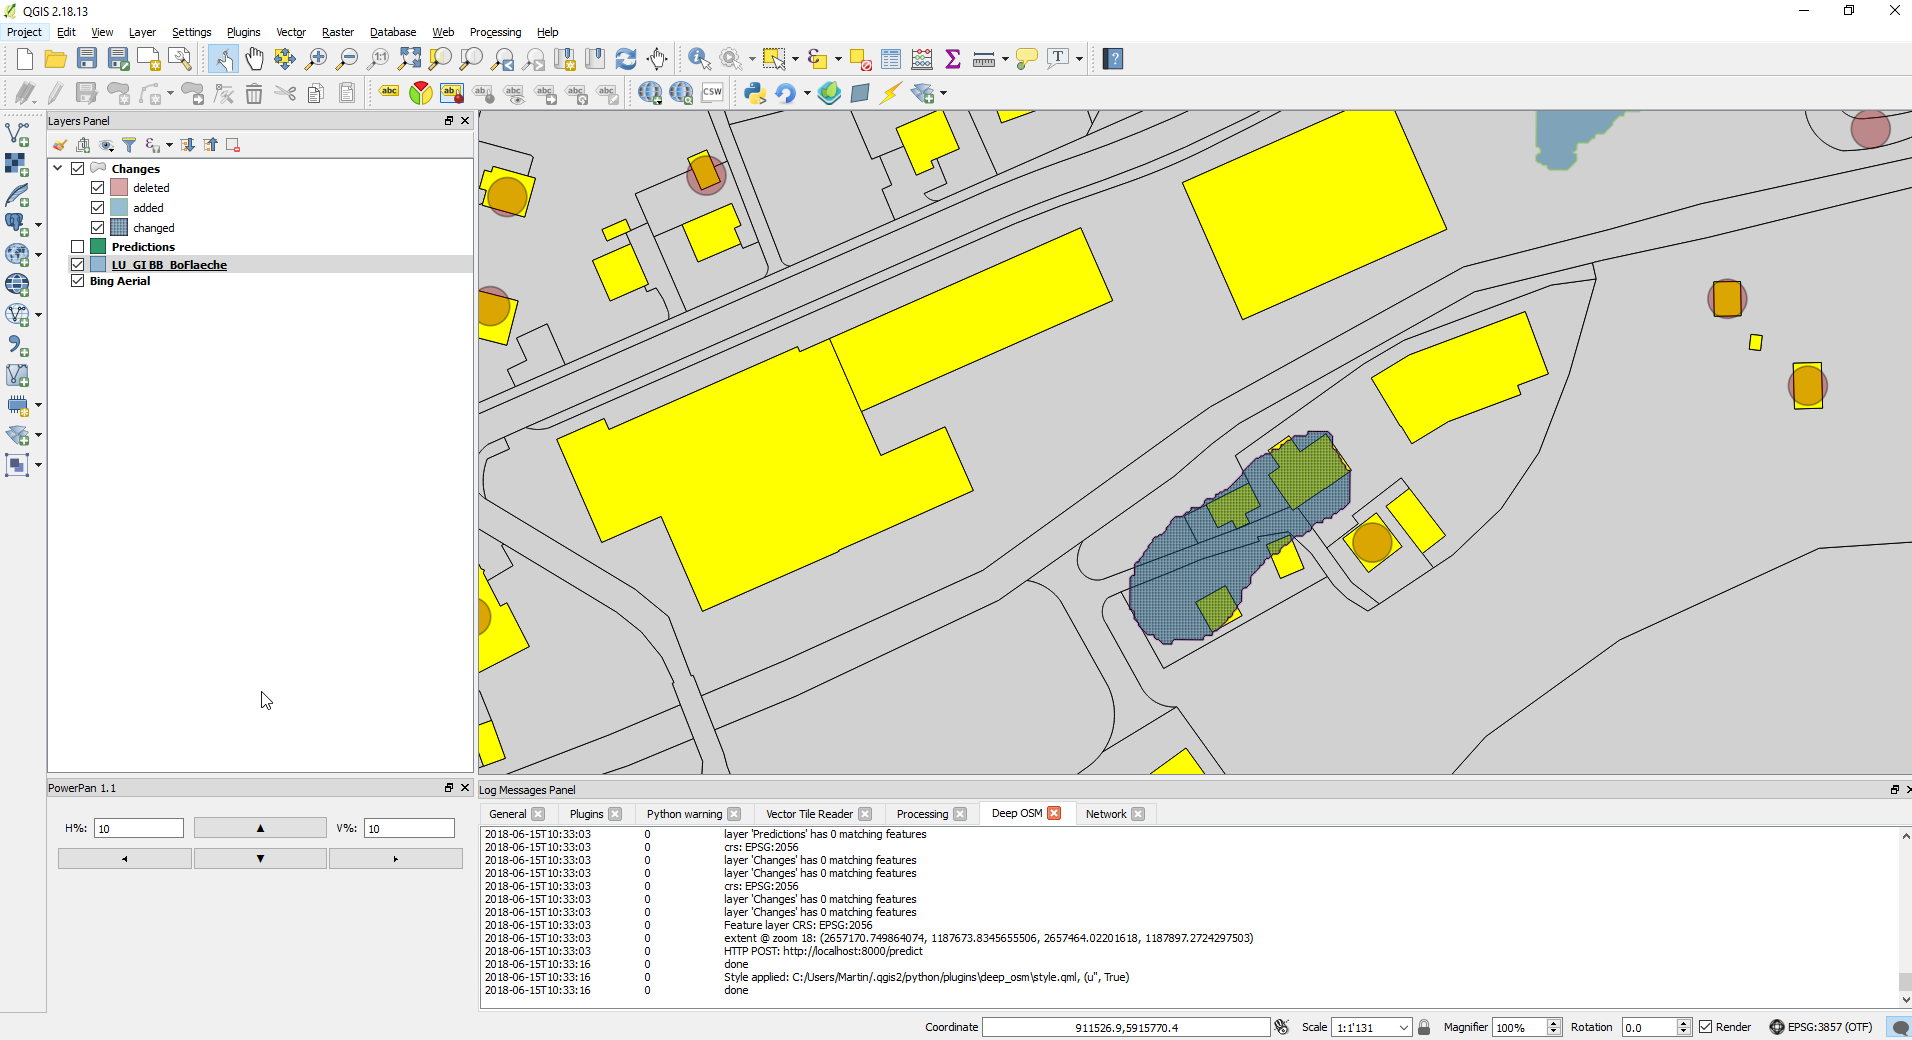
\includegraphics[width=1\linewidth]{chapters/practical_results/images/qgis_changes.png}
	\caption{Changes on cadastral survey data layer}
	\label{fig:plugin:changes_cadastral_layer}
\end{figure}

\begin{figure}[H]
    \centering
	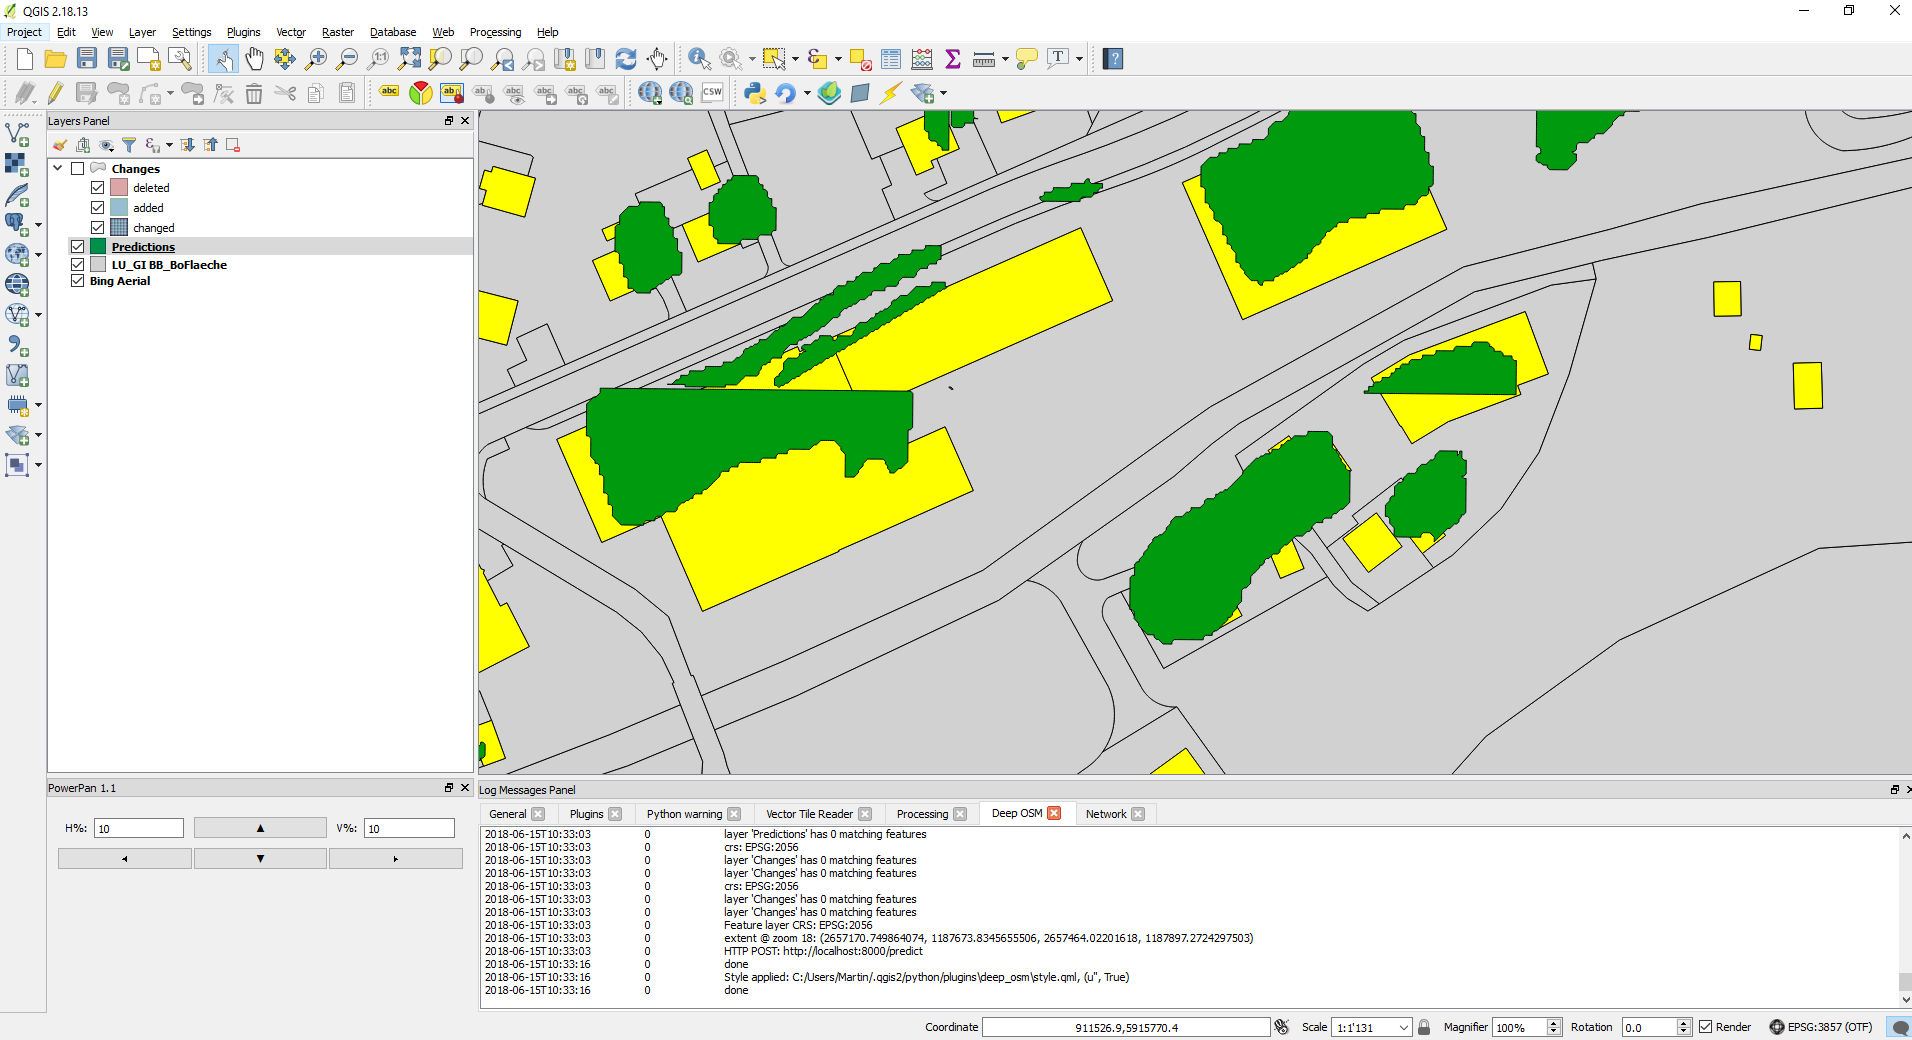
\includegraphics[width=1\linewidth]{chapters/practical_results/images/qgis_predictions.png}
	\caption{Predictions (green) generated by the neural network}
	\label{fig:plugin:predictions}
\end{figure}

\begin{figure}[H]
    \centering
	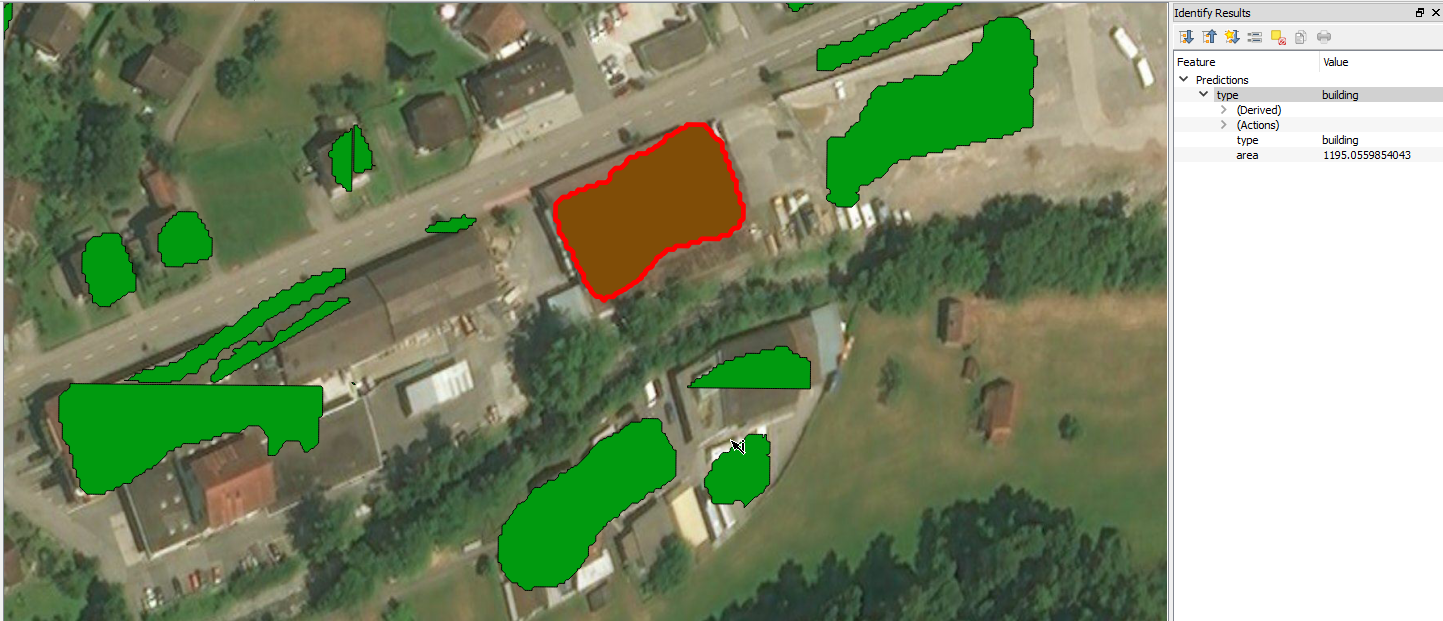
\includegraphics[width=1\linewidth]{chapters/practical_results/images/qgis_prediction_attributes.png}
	\caption{Prediction attributes show the predicted class (here, buildings)}
	\label{fig:plugin:prediction_attributes}
\end{figure}

\begin{figure}[H]
    \centering
	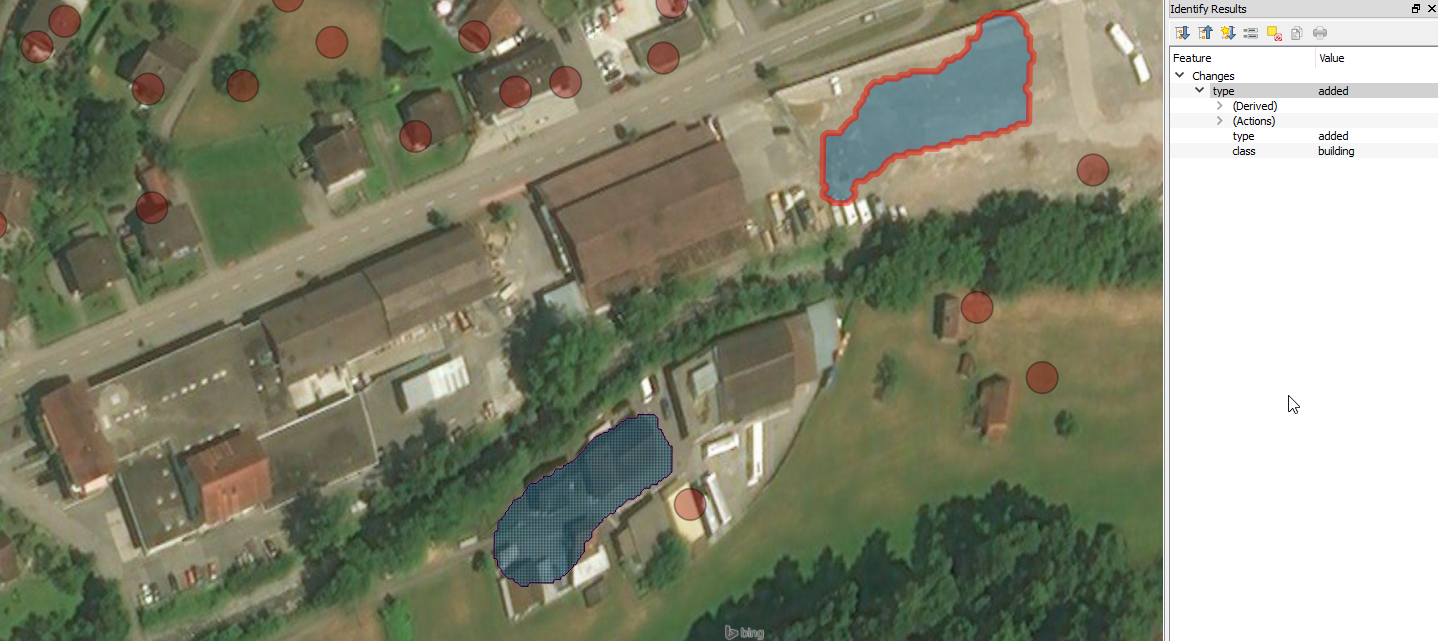
\includegraphics[width=1\linewidth]{chapters/practical_results/images/qgis_changes_attributes.png}
	\caption{Changes have attributes showing the predicted class and type of change (added, deleted, or changed).}
	\label{fig:plugin:change_attributes}
\end{figure}

\section{Prediction Accuracy}
The accuracy of predictions for objects on orthophotos is measured using a method called “intersection over union” (IoU), also known as the Jaccard coefficient \cite{Liu.2011}. The coefficient is a measure of similarity between objects and is calculated as shown in \autoref{fig:results:iou}.

\begin{figure}[H]
    \centering
	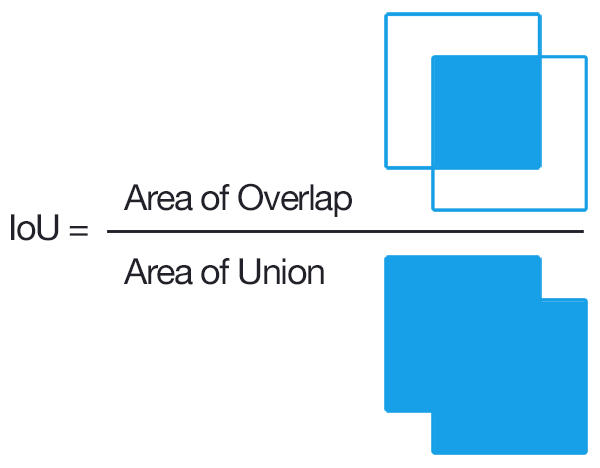
\includegraphics[width=0.6\linewidth]{chapters/practical_results/images/iou_equation.png}
	\caption{The calculation of intersection over union (IoU)\\Source: https://www.pyimagesearch.com/2016/11/07/intersection-over-union-iou-for-object-detection/ (23.06.2018)}
	\label{fig:results:iou}
\end{figure}

However, because of its non-differentiability, the IoU cannot directly be used as a loss-coefficient during the training of the neural network. Nonetheless, there are options for using IoU during training, as reported in literature (\cite{Bebis.2016}, \cite{Yu.20160804}).
The goal of this thesis was not to obtain the most accurate predictions but rather to reduce the false positives and false negatives as much as possible. Hence, it did not matter so much if the prediction was highly accurate but rather that all objects for their corresponding classes should be found. We therefore introduced a new metric, hit rate, which simply counted whether an object was found (hit) or not. It was calculated as follows:

\begin{equation}
	Precision = \dfrac{|TP|}{|TP| + |FP|}
\end{equation}
and
\begin{equation}
	Recall = \dfrac{|TP|}{|TP| + |FN|}
\end{equation}
where:
\begin{itemize}[label=]
    \item $TP$: True positive prediction
    \item $FP$: False positive prediction
    \item $FN$: False negative prediction
\end{itemize}

Finally, accordingly to this metrics, our predictions had a \textbf{Precision of 95.33\%} and a \textbf{Recall of 88.96\%}. These values were obtained using a randomly selected batch of 150 images from the test data set.

